%% ============================================================
%% 分片 23：原文第 9 节「't Hooft And Hecke Operators」（原文 glshort.tex 起于第 6755 行）
%% 由 tools/harvmac2tex.py 从 arXiv 源码（hep-th/0604151v3）自动生成。
%% 只译英文散文；公式、编号、\label、\cite 一律不改。
%% ============================================================

\subsection{'t Hooft Operators And Hecke Modifications}

\label{sec:theck}

To begin with, we consider the Bogomolny equations on
$W=\Bbb{R}^3$, which we regard  as $\Bbb{R}\times\Bbb{C}$, where
$\Bbb{C}$ is parametrized by $z=x^2+ix^3$, and $\Bbb{R}$ by
$y=x^1$.  We have % 式 (9.6)
\setcounter{equation}{5}
\begin{equation}\label{eq:boffo}
\begin{aligned}\star dy&={i\over 2}dz\wedge
d\bar z\\
        \star dz&=-idz\wedge dy\\
        \star d\bar z& = id\bar z\wedge dy.\\\end{aligned}
\end{equation}

        Upon expanding $F=dz\wedge d\bar z \,F_{z\bar z}+dy\wedge dz
        F_{yz}+dy\wedge d\bar z F_{y\bar z}$, and similarly
        $D\phi_0=dy D_y\phi_0+dz D_z\phi_0+d\bar z D_{\bar z}\phi_0$,
the Bogomolny equations become % 式 (9.7)
\setcounter{equation}{6}
\begin{equation}\label{eq:noffo}
\begin{aligned}F_{z\bar
z}&={i\over 2}D_y\phi_0\\
                    F_{yz}&=iD_z\phi_0\\
                    F_{y\bar z}&=-iD_{\bar z}\phi_0.\\\end{aligned}
\end{equation}

More generally, take $W= \Bbb{R}\times C$, with a Riemann surface
$C$. We write $z$ for a local complex coordinate on $C$, endow $C$
with a Kahler metric $h(z,\bar z)|dz|^2$, for some positive
function $h$, and take the metric on $W$ to be $h(z,\bar
z)|dz|^2+dy^2$. The first equations in \eqref{eq:boffo}\ and \eqref{eq:noffo}\ become
respectively % 式 (9.8)
\setcounter{equation}{7}
\begin{equation}\label{eq:jungol}
\begin{aligned}\star dy& ={ih\over 2}\,dz\wedge
d\bar z\\ F_{z\bar z}&={ih\over 2}D_y\phi_0.\end{aligned}
\end{equation}
 The other
equations are unchanged.

There is no integrability condition for $\bar\partial $ operators
in complex dimension 1.  So any connection $A$ on a $G$-bundle
$E\to C$ endows $E$ with a holomorphic structure.  We simply
define the $\bar \partial$ operator as $\bar D=d\bar z D_{\bar
z}=d\bar z(\partial_{\bar z}+A_{\bar z})$.

\begin{figure}[htbp]
\centering
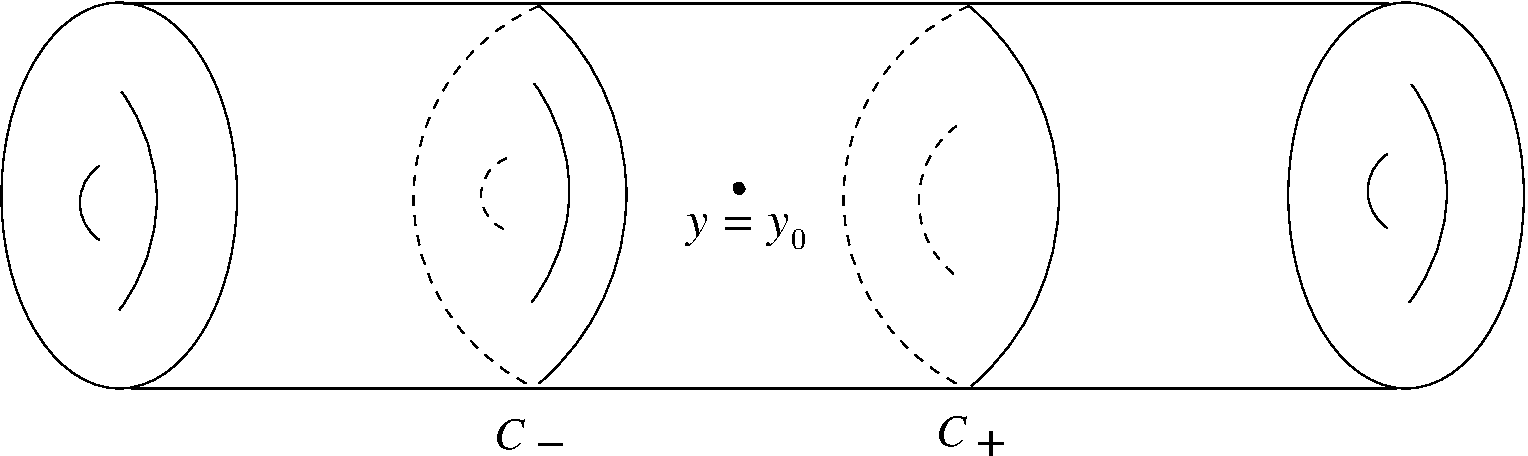
\includegraphics[width=0.75\linewidth]{figures/gla7-2.png}
\caption{In a solution of the Bogomolny equations on a $G$-bundle $E$, the holomorphic type of $E_y$ -- the restriction of $E$ to $ \{y\}\times C$ -- is constant except when one crosses the position of an 't Hooft operator. Sketched are an 't Hooft operator at $y=y_0$ and copies of $C_y=\{y\}\times C$ to the left and right of $y_0$. They are denoted $C_-$ and $C_+$.（原文 Fig.~13）}
\label{fig:otampo}
\end{figure}

Thus, as $y$ varies in $ \Bbb{R}$, any connection $A$ on a
$G$-bundle $E\to  \Bbb{R}\times C$ defines a family of holomorphic
$G$-bundles $E_y\to C$. $E_y$ is simply the restriction of $E$ to
$C_y= \{y\}\times C$ (\otampo). Now suppose that $A$ obeys the
Bogomolny equations. Let us work in the gauge $A_y=0$. Then
$F_{y\bar z}=\partial_yA_{\bar z}$. Hence the last equation in
\eqref{eq:noffo}\ tells us that % 式 (9.9)
\setcounter{equation}{8}
\begin{equation}\label{eq:troffo}
{\partial\over
\partial y}A_{\bar z}=-iD_{\bar z}\phi_0.
\end{equation}

But the right hand side is the change in $A_{\bar z}$ under a
gauge transformation generated by $-i\phi_0$.  Hence the
holomorphic type of $E_y$ is independent of $y$.  (Another way to
state this argument is to note that $\partial_y\bar D=-i[\bar
D,\phi_0]$, showing that $\bar D$ is independent of $y$ up to
conjugation.)

Now let us see what happens if we incorporate an 't Hooft operator
at a point $p=y_0\times p_0\in \Bbb{R}\times C$. This means that
we consider a bundle $E$ and connection $A$ that are defined on
the complement of the point $p$, and which have a certain type of
singularity near $p$, as described in section 第~\ref{sec:tophooft}~节.

Away from $y=y_0$, the above argument applies and the holomorphic
type of $E_y$ is independent of $y$.  At $y=y_0$, because of the
singularity, the bundle $E_y$ is not defined.  In crossing
$y=y_0$, the holomorphic type of the bundle may jump.  However, it
can only jump in a very special way.  If we restrict $E$ to
$C\backslash p_0$ (that is, the complement of $p_0$ in $C$), then
the above argument applies and the restricted bundle $E_y$ has a
holomorphic type that is constant even at $y=y_0$.  So the
holomorphic type of $E_y$ may jump at $y=y_0$, but only in a way
that is trivial if we omit the point $p_0$ from $C$.

We will now try to describe precisely how $E_y$ can jump at
$y=y_0$.  We consider first the abelian case, and then the
nonabelian case.

\par\medskip{\it The Abelian Case}

We begin with $G=U(1)$.  In this case, $E$ is a complex line
bundle ${\cal L}$. We write ${\cal L}_-$ for ${\cal L}_y$ with
$y<y_0$ and ${\cal L}_+$ for ${\cal L}_y$ with $y>y_0$.  The line
bundles ${\cal L}_-$ and ${\cal L}_+$ are isomorphic on the
complement of the point $p_0\in C$.

This means that the line bundle ${\cal L}_+\otimes {\cal
L}_-^{-1}$ is trivial away from $p_0$.  It hence has a section $s$
that has neither a zero nor a pole away from $p_0$; let $q$ be the
order of its zero at $p_0$.  Then ${\cal L}_+\otimes {\cal
L}_-^{-1}\cong {\cal O}(p_0)^q$.  Here as usual ${\cal O}(p_0)$ is
the line bundle whose holomorphic sections are  functions
holomorphic away from $p_0$ with a possible single pole at $p_0$.
So the relation between ${\cal L}_+$ and ${\cal L}_-$ is ${\cal
L}_+\cong {\cal L}_-\otimes {\cal O}(p_0)^q$, for some integer
$q$.

We recall that an 't Hooft operator $T(m)$ for the group $G=U(1)$
is classified by the choice of an integer $m$. (We write the
operator as $T(m;p_0)$ if we want to specify the point $p_0$.)
This suggests an obvious hypothesis -- that $m$ may coincide with
the integer $q$ of the last paragraph.

The operator $T(m)$ is defined by saying that near $p=p_0\times
y_0$, the curvature has the singular behavior % 式 (9.10)
\setcounter{equation}{9}
\begin{equation}\label{eq:formigo}
F\sim
\star d\left({im\over 2}{1\over |\vec x - p|}\right),
\end{equation}
 where
$|\vec x-p|$ is the distance from $p$ to a nearby point $\vec x\in
 \Bbb{R}\times C$.  This implies that if $S$ is a small sphere enclosing
the point $p$, as in the figure, then $\int_S c_1({\cal L})=m$.
The 't Hooft operators $T(m)$ are thus all topologically distinct
from one another.  This statement, which is far from being valid
if $G$ is nonabelian,   will enable us in the abelian case to
determine the action of $T(m)$ just on topological grounds.

\begin{figure}[htbp]
\centering
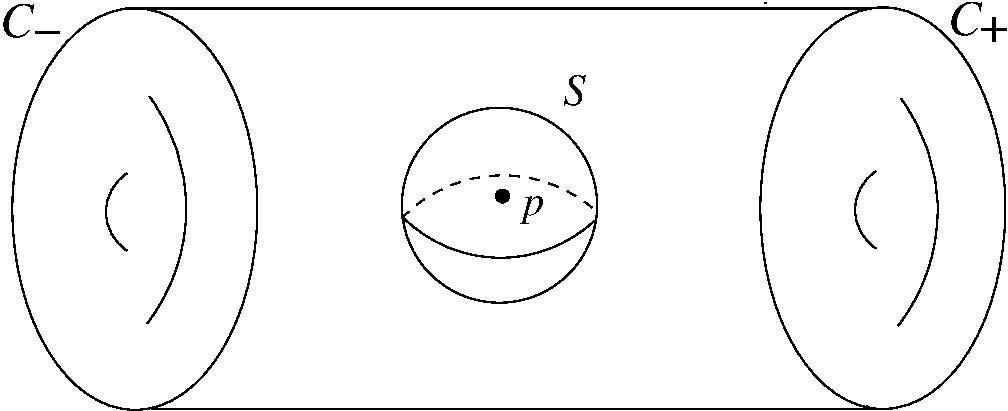
\includegraphics[width=0.75\linewidth]{figures/gla7-3.png}
\caption{A cobordism between the two-cycles $C_-+S$ and $C_+$, showing that the homology cycle $D=C_+-C_--S$ is a boundary.（原文 Fig.~14）}
\label{fig:notampo}
\end{figure}

 Now pick $y_\pm$ with
$y_-<y_0<y_+$, and write $C_\pm$ for $ y_\pm\times C$, so that
${\cal L}_\pm $ is the restriction of ${\cal L}$ to $C_\pm$. Let
$q_\pm=\int_{C_\pm}c_1({\cal L})$. With an obvious choice of
orientations, as in  \notampo, the homology cycle $D=C_+-C_--S$ is
a boundary in $(\Bbb{R}\times C)\backslash p$. Hence
$0=\int_Dc_1({\cal L})=\int_{C_+}c_1({\cal L})-\int_{C_-}c_1({\cal
L})-\int_Sc_1({\cal L})=q_+-m-q_-$.

So $q_+=m+q_-$.  Consequently, ${\cal L}_+$ and ${\cal L}_-$,
which are isomorphic away from $p_0$, differ in first Chern class
by $m$. Hence ${\cal L}_+\cong {\cal L}_-\otimes {\cal O}(p_0)^m$.

Thus, we have determined the action of the 't Hooft operators for
$G=U(1)$.  The 't Hooft operator $T(m;p_0)$, that is the operator
$T(m)$ inserted at the point $p_0\in C$, acts by twisting with
${\cal O}(p_0)^m$.   This result agrees with the standard
definition of the Hecke operators for $U(1)$.

We see that, in accord with general arguments in section 第~\ref{sec:lineop}~节,
 't Hooft operators inserted at distinct points in $C$
 commute.  Moreover, the 't Hooft operators at
a given point $p_0\in C$ form a commutative group, with
$T(m;p_0)=T(1;p_0)^m$.

\par\medskip{\it The Nonabelian Case: $U(N)$}

\def\VV{\eurm V}

Now let us discuss what 't Hooft operators do in the nonabelian
case.  We first consider the group $U(N)$.  There are two things
that make this group simple to analyze.  $U(N)$ has a convenient
representation, the $N$-dimensional representation that we will
call $\VV$. And $U(N)$ is its own Langlands dual.

The definition of an 't Hooft operator depends on a choice of
homomorphism $\rho:U(1)\to U(N)$, up to conjugation.  The most
general such homomorphism maps $\exp({i\alpha})\in U(1)$ to the
diagonal matrix ${\rm
diag}(\exp({im_1\alpha}),\exp({im_2\alpha}),\dots,
\exp({im_N\alpha}))$, with an $N$-plet of integers
$^L\negthinspace w=(m_1,m_2,\dots,m_N)$ that are unique up to
permutation. (We call this quantity $^L\negthinspace w$ because in
the general case, it will be a weight of the dual group
$^L\negthinspace G$.) We will usually order the $m_i$ so $m_1\geq
m_2\geq \dots\geq m_N$. At the Lie algebra level, $\rho$ maps
$1\in \frak{u}(1)$ to the diagonal matrix
% 式 (9.11)
\setcounter{equation}{10}
\begin{equation}\label{eq:morphy}
\left(\begin{matrix}m_1& & & \dots & \\
                                    &m_2& & \dots & \\
                          & & m_3 &\dots & \\
                & & \vdots & \dots& \\
            & & & & m_N\\\end{matrix}\right).
\end{equation}

The corresponding 't Hooft operator $T(^L\negthinspace w)$ is
defined by saying that near the point $p\in  \Bbb{R}\times C$, the
gauge field has a singularity obtained by embedding the basic
$U(1)$ singularity in $U(N)$, via this embedding.  For example,
the singular part of the curvature near $p$ is diagonal
% 式 (9.12)
\setcounter{equation}{11}
\begin{equation}\label{eq:orphy}
F\sim \star d\left({i\over 2}{1\over |\vec x -
p|}\right) \left(\begin{matrix}m_1& & & \dots & \\
                                    & m_2& & \dots & \\
                          & & m_3 &\dots & \\
                & & \vdots & \dots& \\
            & & & & m_N\\\end{matrix}\right).
\end{equation}

Near $p$, the Bogomolny equations reduce to equations in some
maximal torus ${\cal T}=U(1)^N$ of $U(N)$. (From a holomorphic
point of view, it is more natural to consider the corresponding
reduction to a complexified maximal torus in the complexification
of the gauge group, namely $U(N)_{\Bbb{C}}=GL(N,\Bbb{C})$.)
Corresponding to the reduction of the equations to a maximal
torus, the bundle $E_y$ splits up, near $p_0\times y \in C_y$, as
a sum ${\cal L}_1\oplus {\cal L}_2\oplus\dots \oplus {\cal L}_N$
of line bundles (each of which, of course, is trivial near $p$).
The effect of the 't Hooft operator on ${\cal L}_i$ is precisely
what it was in the abelian case, namely ${\cal L}_i\to {\cal
L}_i\otimes {\cal O}(p_0)^{m_i}$.

Thus, we have arrived at a description of how the 't Hooft
operator $T(^L\negthinspace w)$  acts on a bundle $E$.  Relative
to some decomposition of $E$ as $\oplus_{i=1}^N{\cal L}_i$ near
$p$, it acts by ${\cal L}_i\to {\cal L}_i\otimes {\cal
O}(p_0)^{m_i}$. This coincides with the usual mathematical
description of the action of the Hecke operators for $U(N)$.
This is the basic link between 't Hooft and Hecke operators.

In sections 第~\ref{sec:spaceheck}~节\ and 第~\ref{sec:affgrass}~节, we will address the
question of what sort of data is contained in the local
decomposition of $E$ as $\oplus_{i=1}^N{\cal L}_i$, and how much
of this data is relevant to the action of the 't Hooft operators.
The general answer to this question involves something called the
affine Grassmannian, which we briefly describe in section
第~\ref{sec:affgrass}~节.

\par\medskip{\it Some Examples}

In general, as we know from section 第~\ref{sec:tophooft}~节, representations of
the Langlands dual group $^L\negthinspace G$ correspond naturally
to 't Hooft operators of $G$. A representation $R(^L\negthinspace
w)$ with highest weight $^L\negthinspace w$ corresponds to an 't
Hooft operator that we write as $T(R(^L\negthinspace w))$ or
simply as $T(^L\negthinspace w)$. In the present discussion,
$^L\negthinspace G=G=U(N)$.

For example, the fundamental $N$-dimensional representation $\VV$
of $U(N)$ has, with our convention $m_1\geq m_2\geq \dots\geq
m_N$, the highest weight $^L\negthinspace w(1)=(1,0,0,\dots,0)$.
It corresponds to an 't Hooft operator $T(^L\negthinspace w(1))$
or simply $T_{(1)}$. The $k^{th}$ antisymmetric tensor
representation $\wedge^k\VV$, for $k=1,\dots,N$, has highest
weight % 式 (9.13)
\setcounter{equation}{12}
\begin{equation}\label{eq:nyto}
^L\negthinspace
w(k)=(\overbrace{1,1,\dots,1}^{\text {$k$ times}},0,\dots,0)
\end{equation}
 and
corresponds to an 't Hooft operator $T_{(k)}$.

The representation $\wedge^N\VV$ is one-dimensional; it is the
representation in which $g\in U(N)$ acts by multiplication by
$\det(g)$.  It can be raised to any integer power $u$, positive or
negative, to get a representation in which $g$ acts by
$(\det(g))^u$. This representation, which we denote as
$(\wedge^N\VV)^u$, corresponds to the weight $^L\negthinspace
w=(u,u,\dots,u)$. The 't Hooft/Hecke operator $T_{(N)}$
corresponding to $\wedge^N\VV$ simply acts by $E\to E\otimes {\cal
O}(p_0)$, as in the abelian case, and is obviously invertible. Its
$u^{th}$ power corresponds to the representation
$(\wedge^N\VV)^u$.  The $T_{(k)}$ with $k<N$ are not invertible.

The central element $\exp(i\alpha)$ of $U(N)$ acts on the
representation $\wedge^k\VV$ as multiplication by
$\exp(ik\alpha)$. More generally, it acts on any representation of
highest weight $^L\negthinspace w=(m_1,m_2,\dots,m_N)$ as
multiplication by $\exp(i\alpha\sum_{i=1}^Nm_i)$. A special case
of this statement is that the center of $U(N)$ acts trivially if
and only if % 式 (9.14)
\setcounter{equation}{13}
\begin{equation}\label{eq:hoty}
\sum_im_i=0.
\end{equation}
 $S$-duality, as we discussed
in section 第~\ref{sec:electricbranes}~节, maps the action of the center of
$^L\negthinspace G$ on a representation $^L\negthinspace R$ to the
action of the corresponding 't Hooft operator $T(^L\negthinspace
R)$ on the topology of a $G$-bundle.  Indeed, since
$T(^L\negthinspace w)$ locally maps $\oplus_i{\cal L}_i$ to
$\oplus_i\left({\cal L}_i\otimes {\cal O}(p_0)^{m_i}\right)$, it
changes $c_1(E)$ by % [WARN] 公式 \eqn\eqref{eq:yorgo} 无编号或重复
\begin{equation*}
\tag*{(9.15)}
c_1(E)\to c_1(E)+\sum_im_i,
\end{equation*}
 and
thus the topology of $E$ is unchanged if and only if
$\sum_im_i=0$.

{}From $S$-duality, we expect 't Hooft operators of $G$ to form a
commutative algebra isomorphic to the representation ring of
$^L\negthinspace G$.  (In fact, as we discussed in section
第~\ref{sec:lineop}~节, commutativity of 't Hooft operators follows from more
general considerations of four-dimensional topological field
theory, without resort to $S$-duality.)  We will examine this in
section 第~\ref{sec:kahstr}~节\ from the standpoint of the Bogomolny equations.
The representation ring of $U(N)$ is freely generated by the
representations $\wedge ^k\VV,\,k=1,\dots,N$ along with
$(\wedge^N\VV)^{-1}$. Accordingly the commutative algebra of 't
Hooft operators for $U(N)$ is freely generated by the $T_{(k)}$
together with $T_{(N)}^{-1}$. In the mathematical literature on
the geometric Langlands program, these generators are usually
taken as the basic Hecke operations of $U(N)$.

\par\medskip{\it 't Hooft/Hecke Operators For Other Groups}

The generalization of this to any compact gauge group $G$ is
rather direct. To keep things relatively simple, we will pick a
representation $R$ of $G$ and and consider a $G$-bundle $E_R$
which we take in the representation $R$. (Thus, if $E$ denotes a
principal $G$-bundle, then $E_R=E\times_G R$.) Picking a maximal
torus ${\cal T}$  of $G$, let $w$ denote a weight of $G$, that is
a character $w:{\cal T}\to U(1)$. Let $R=\oplus_wR_w$ be the
decomposition of $R$ in weight spaces $R_w$ (all but finitely many
of which vanish).

An 't Hooft operator of $G$ is classified by a dominant coweight
$^L\negthinspace w:U(1)\to {\cal T}$, which is the highest weight
of a representation $^L\negthinspace R$ of $^L\negthinspace G$.
The composition  of $w:{\cal T}\to U(1)$ and $ ^L\negthinspace
w:U(1)\to {\cal T}$ is a homomorphism $w\circ{}^L\negthinspace
w:U(1)\to U(1)$ which takes the form $\exp(i\alpha)\to
\exp(i\langle ^L\negthinspace w,w\rangle\alpha)$ for some integer
$\langle ^L\negthinspace w,w\rangle$.

For any choice of a complexified maximal torus ${\cal
T}_{\Bbb{C}}$ of $G_{\Bbb{C}}$, the fiber of $E_R$ at $p_0\in C$
has a decomposition $E_R|_{p_0}=\oplus_w E_{R,w}|_{p_0}$ in weight
spaces. If we extend ${\cal T}$ to a holomorphically varying
family of maximal tori near $p_0$, then we get a corresponding
local decomposition of $E_R$ in subbundles of definite weight:
$E_R=\oplus_w {E}_{R,w}$. By solving the Bogomolny equations near
$p_0$, and taking account of the abelian nature of the
singularity, we find that relative to some choice of such a
decomposition, $T(^L\negthinspace w)$ acts by ${E}_{R,w}\to {
E}_{R,w}\otimes {\cal O}(p_0)^{\langle ^L\negthinspace
w,w\rangle}$.

We will make this more concrete for the case $G=SU(N)$,
$^L\negthinspace G=PSU(N)=SU(N)/\Bbb{Z}_N$, and the reciprocal
case $G=PSU(N)$, $^L\negthinspace G=SU(N)$.

A homomorphism $\rho:U(1)\to G=SU(N)$ takes the same form as for
$U(N)$, namely $\exp(i\alpha)\to{\rm
diag}(\exp({im_1\alpha}),\exp({im_2\alpha}),\dots,\exp(im_N\alpha))$,
except that now we must require $\sum_im_i=0$, as in \eqref{eq:hoty}.  The
action of the corresponding 't Hooft operator $T(^L\negthinspace
w)$ on an $SU(N)$ bundle $E$ is as before: relative to some
decomposition $E=\oplus_{i=1}^N{\cal L}_i$ near $p$, we have
${\cal L}_i\to {\cal L}_i\otimes {\cal O}(p_0)^{m_i}$.

With our usual ordering $m_1\geq m_2\geq\dots\geq m_N$, the
$N$-plet $^L\negthinspace w=(m_1,m_2,\dots,m_N)$ is a positive
integer combination of the simple roots $e_1=(1,-1,0,\dots,0)$,
$e_2=(0,1,-1,0,\dots,0),\dots ,e_{N-1}=(0,0,\dots,0,1,-1)$ of
$SU(N)$. Hence, it is the highest weight of a representation of
the adjoint group $PSU(N)$, which of course coincides with
$^L\negthinspace G$ in this case.

Now let us discuss the case that $G=PSU(N)$, and therefore
$^L\negthinspace G=SU(N)$.  A homomorphism $\rho:U(1)\to PSU(N)$
can be lifted to a homomorphism from an $N$-fold cover of $U(1)$
to $SU(N)$. Such a homomorphism takes the form $\exp(i\alpha)\to
{\rm
diag}(\exp(im_1\alpha),\exp(im_2\alpha),\dots,\exp(im_N\alpha))$,
but the $m_i$ are not integers; rather, they take values in
 ${1\over N}\Bbb{Z}$, with the differences $m_i-m_j$ being integers. Such an $N$-plet
$^L\negthinspace w=(m_1,m_2,\dots,m_N)$, ordered so that $m_1\geq
m_2\geq \dots\geq m_N$, is a dominant weight of $^L\negthinspace
G=SU(N)$. It corresponds to a representation $^L\negthinspace R$
of $SU(N)$ and an 't Hooft operator $T(^L\negthinspace R)$ of
$G=PSU(N)$. The representations $^L\negthinspace R$ on which the
center of $SU(N)$ acts nontrivially, and hence those for which
$T(^L\negthinspace R)$ changes the topology of a $PSU(N)$-bundle,
are precisely those for which the $m_i$ are non-integral.

Let $E$ be a principal $PSU(N)$ bundle.  As $PSU(N)$ does not have
an $N$-dimensional representation corresponding to the
$N$-dimensional representation $\VV$ of $SU(N)$, we cannot derive
from $E$ a rank $N$ complex vector bundle $E_\VV$.  However,
$E_\VV$ does exist as a twisted vector bundle, a notion that we
explained briefly  in section 第~\ref{sec:comptwop}~节.  The obstruction to
lifting $E_\VV$ to an ordinary vector bundle is the characteristic
class $\xi(E)$ introduced in section 第~\ref{sec:reviewthis}~节.  After picking a
family of maximal tori, $E_\VV$ has a local decomposition
$E_\VV=\oplus_{i=1}^N{\cal L}_i$ in terms of twisted line bundles
${\cal L}_i$ (all of which are twisted in the same way, since the
obstruction to lifting $E_\VV$ to a vector bundle is central).

The 't Hooft/Hecke operators act, relative to some such
decomposition, in the familiar way  ${\cal L}_i\to{\cal
L}_i\otimes {\cal O}(p_0)^{m_i}$.  Now, however, the $m_i$ may not
be integers.  We define ${\cal O}(p_0)^{1/N}$ as a twisted line
bundle, and we define ${\cal O}(p_0)^{m/N}$, for any integer $m$,
as the $m^{th}$ power of ${\cal O}(p_0)^{1/N}$.  In particular,
the $N^{th}$ power of ${\cal O}(p_0)^{1/N}$ is the ordinary line
bundle ${\cal O}(p_0)$.  Since the differences $m_i-m_j$ are
integers, the twisted line bundles ${\cal O}(p_o)^{m_i}$ are all
twisted in the same way, and the action of the 't Hooft/Hecke
operators by ${\cal L}_i\to {\cal L}_i\otimes {\cal O}(p_0)^{m_i}$
preserves the fact that the ${\cal L}_i$ all have the same twist.

Of course, we can avoid talking about twisted bundles by picking a
representation $R$ of $PSU(N)$, and applying the 't Hooft
operators to the ordinary vector bundle $E_R=E\times_{PSU(N)}R$.
For example, let $N=2$, so that $PSU(2)$ becomes $SO(3)$. The rank
two twisted bundle $E_\VV$ has the local decomposition ${\cal
L}\oplus {\cal L}^{-1}$ in terms of a twisted line bundle ${\cal
L}$. If we take $R$ to be the adjoint representation of $SO(3)$,
then the corresponding adjoint bundle $E_R$ is ${\rm
Sym}^2(E_\VV)$ (the symmetric part of $E_\VV\otimes E_\VV$) or
${\cal L}^2\oplus {\cal O}\oplus {\cal L}^{-2}$, where ${\cal
L}^2$ is an ordinary line bundle.  The transformation ${\cal L}\to
{\cal L}\otimes {\cal O}(p_0)^{1/2}$ acts on $E_R$  by $E_R\to
({\cal L}^2\otimes \CO(p_0))\oplus \CO\oplus ({\cal L}^{-2}\otimes
\CO(p_0)^{-1})$.  This transformation involves no fractional
exponents.
